\chapter{Introducción}
\label{cap:capitulo1}
\setcounter{page}{1}

\begin{flushright}
\begin{minipage}[]{10cm}
\emph{La motivación nos impulsa a comenzar y el hábito nos permite continuar}\\
\end{minipage}\\

Jim Ryun\\
\end{flushright}

\vspace{1cm}

La robótica ha sufrido una transformación enorme a lo largo de su historia aunque siempre teniendo en mente el mismo objetivo: cumplir con el deseo humano. Debido a esa transformación y ese deseo, se ha podido consolidar este campo en la actualidad que abarca cada sector que se pueda imaginar. Otra vertiente que ha destacado en la robótica estos últimos años ha sido la creación de robots de bajo coste para que puedan llegar a un mayor número de personas y se puedan beneficiar de esta ciencia. 

En el presente capítulo se va a abordar el contexto de la robótica, explicando brevemente su historia para poder entender realmente qué es la robótica y lo que es un robot. También se van a encuadrar los tipos de robots que existen y sus múltiples aplicaciones. Todo esto nos ayudará a poder entender mejor dónde se encuadra el presente trabajo, proporcionando los conocimientos necesarios, tanto teóricos como prácticos, que se describirán a lo largo del documento.\\

\section{La robótica}
\label{sec:robotica} % etiqueta para luego referenciar esta sección

La robótica es el campo de la ingeniería que se enfoca en el diseño, la construcción y la programación de robots para tareas específicas. Por ende, un robot se podría definir como un sistema informático formado por sensores, actuadores y computadores imprecisos, ya que tienen ruido. Los robots realizan tareas sucias, aburridas y peligrosas y tienen que ser sensibles al entorno. Sin embargo, no existe una definición unívoca al respecto y depende del campo y de la época de la que queramos hablar. Para ello, se va a hacer un breve resumen sobre la historia de la robótica.

En los textos puedes poner palabras en \textit{cursiva}, para aquellas expresiones en sentido \textit{figurado}, palabras como \textit{robota}, que está fuera del diccionario castellano, o bien para resaltar palabras de una colección: \textit{(a)} es la primera letra del abecedario, \textit{(b)} es la segunda, etc.\\

Al poner las dos líneas del anterior párrafo, este aparecerá separado del anterior. Si no las pongo, los párrafos aparecerán pegados. Sigue el criterio que consideres más oportuno.

\section{Segunda sección}
\label{sec:segundaseccion}

No olvides incluir imágenes y referenciarlas, como la Figura \ref{fig:roomba}.

\begin{figure} [h!]
  \begin{center}
    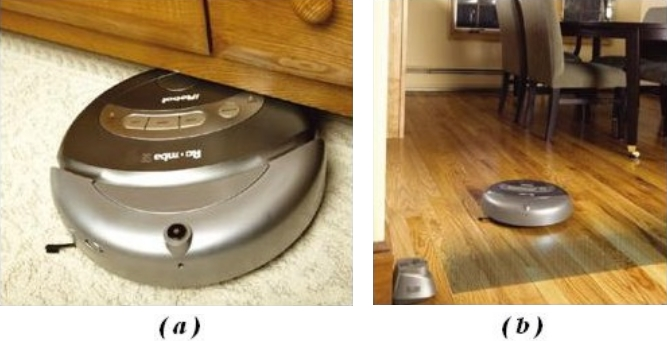
\includegraphics[width=8cm]{figs/roomba}
  \end{center}
  \caption{Robot aspirador Roomba de iRobot.}
  \label{fig:roomba}
\end{figure}\

Ni tampoco olvides de poner las URLs como notas al pie. Por ejemplo, si hablo de la Robocup\footnote{\url{http://www.robocup.org}}.

\subsection{Números}
\label{sec:subseccion}

En lugar de tener secciones interminables, como la Sección \ref{sec:miseccion}, divídelas en subsecciones.

Para hablar de números, mételos en el entorno \textit{math} de \LaTeX, por ejemplo, $1.5Kg$. También puedes usar el símbolo del Euro como aquí: 1.500\euro.

\subsection{Listas}

Cuando describas una colección, usa \texttt{itemize} para ítems o \texttt{enumerate} para enumerados. Por ejemplo:

\begin{itemize}
 \item \textit{Entorno de simulación.} Hemos usado dos entornos de simulación: uno en 3D y otro en 2D.
 \item \textit{Entornos reales.} Dentro del campus, hemos realizado experimentos en Biblioteca y en el edificio de Gestión.
\end{itemize}\

\begin{enumerate}
 \item Primer elemento de la colección.
 \item Segundo elemento de la colección.
\end{enumerate}\

\paragraph{Referencias bibliográficas}
\label{sec:referencias}

Cita, sobre todo en este capítulo, referencias bibliográficas que respalden tu argumento. Para citarlas basta con poner la instrucción \verb|\cite| con el identificador de la cita. Por ejemplo: libros como \cite{vega12e}, artículos como \cite{vega19b}, URLs como \cite{vega19a}, tesis como \cite{vega18b}, congresos como \cite{vega18a}, u otros trabajos fin de grado como \cite{vega08b}.

Las referencias, con todo su contenido, están recogidas en el fichero \texttt{bibliografia.bib}. El contenido de estas referencias está en formato \texttt{BibTex}. Este formato se puede obtener en muchas ocasiones directamente, desde plataformas como \texttt{Google Scholar} u otros repositorios de recursos científicos.

Existen numerosos estilos para reflejar una referencia bibliográfica. El estilo establecido por defecto en este documento es APA, que es uno de los estilos más comunes, pero lo puedes modificar en el archivo \texttt{memoria.tex}; concretamente, cambiando el campo \verb|apalike| a otro en la instrucción \verb|\bibliographystyle{apalike}|. 

\

\

\

Y, para terminar este capítulo, resume brevemente qué vas a contar en los siguientes.
